% Created 2016-11-24 Do 12:43
\documentclass[a4paper]{scrartcl}
\usepackage[utf8]{inputenc}
\usepackage[T1]{fontenc}
\usepackage{fixltx2e}
\usepackage{graphicx}
\usepackage{longtable}
\usepackage{float}
\usepackage{wrapfig}
\usepackage{rotating}
\usepackage[normalem]{ulem}
\usepackage{amsmath}
\usepackage{textcomp}
\usepackage{marvosym}
\usepackage{wasysym}
\usepackage{amssymb}
\usepackage{hyperref}
\tolerance=1000
\usepackage{siunitx}
\usepackage{fontspec}
\sisetup{load-configurations = abbrevations}
\newcommand{\estimates}{\overset{\scriptscriptstyle\wedge}{=}}
\usepackage{mathtools}
\DeclarePairedDelimiter\abs{\lvert}{\rvert}%
\DeclarePairedDelimiter\norm{\lVert}{\rVert}%
\makeatletter
\let\oldabs\abs
\def\abs{\@ifstar{\oldabs}{\oldabs*}}
\let\oldnorm\norm
\def\norm{\@ifstar{\oldnorm}{\oldnorm*}}
\makeatother
\DeclareMathOperator{\Exists}{\exists}
\DeclareMathOperator{\rot}{rot}
\DeclareMathOperator{\Forall}{\forall}
\def\cvec#1{\left(\vcenter{\halign{\hfil$##$\hfil\cr \cvecA#1;;}}\right)}
\def\cvecA#1;{\if;#1;\else #1\cr \expandafter \cvecA \fi}
\renewcommand{\d}{\mathrm{d}}
\newcommand{\f}[2]{\frac{#1}{#2}}
\newcommand{\dd}[2]{\frac{\d #1}{\ d#2}}
\renewcommand{\v}[1]{\vec{#1}}
\usepackage{pgfplots}
\usepackage{amsthm}
\theoremstyle{definition}
\newtheorem{defn}{Definition}
\theoremstyle{plain}
\newtheorem{thm}{Satz}
\theoremstyle{remark}
\newtheorem{remark}{Bemerkung}
\usepackage{etoolbox}
\patchcmd{\thmhead}{(#3)}{#3}{}{}
\usepackage{xparse}% http://ctan.org/pkg/xparse
\NewDocumentCommand{\overarrow}{O{=} O{\uparrow} m}{%
\overset{\makebox[0pt]{\begin{tabular}{@{}c@{}}#3\\[0pt]\ensuremath{#2}\end{tabular}}}{#1}
}
\NewDocumentCommand{\underarrow}{O{=} O{\downarrow} m}{%
\underset{\makebox[0pt]{\begin{tabular}{@{}c@{}}\ensuremath{#2}\\[0pt]#3\end{tabular}}}{#1}
}
\renewcommand*{\proofname}{Beweis}
\newcommand{\I}{\ensuremath{i}}%
\newcommand{\ubar}[1]{\underline{#1}}
\author{Robin Heinemann}
\date{\today}
\title{Theoretische Physik (Hebecker)}
\hypersetup{
  pdfkeywords={},
  pdfsubject={},
  pdfcreator={Emacs 25.1.1 (Org mode 8.2.10)}}
\begin{document}

\maketitle
\tableofcontents

Einleitung: \\
\begin{itemize}
\item Webseite: www.thphys.uni-heidelberg.de/hebecker/TP1/tp1.html
\item Bartelman skripte
\end{itemize}

\section{Semesterüberblick}
\label{sec-1}
\begin{enumerate}
\item Newtonsche Mechanik
\item Lagrange / Hamilton Mechanik / Statistik / Kontinua
\item Elektrodynamik / Spezielle Relativitättheorie
\item Quatenmechanik
\item Thermodynamik / Quantenstatistik
\item Allgemeine Relativitättheorie / Kosmologie
\item Quatenfeldtheorie I (ggf. 5.)
\item Quatenfeldtheorie II (ggf. 6. $\Leftarrow$ Stringtheorie / Teilchenphysik / Supersymmetrie)
\item Masterarbeit
\item Masterarbeit
\end{enumerate}
\subsection{Mathe}
\label{sec-1-1}
\textbf{wichtig:}
\begin{itemize}
\item Gruppentheorie
\item Differientialgeometrie
\end{itemize}
\section{Kinematik des Massenpunktes}
\label{sec-2}
Massenpunkt / Punktmasse - (selbstevidente) Abstraktion
Kinematik: Bescheibung der Bewegung (Ursachen der Bewegung $\rightarrow$ Dynamik)
\subsection{Kinematik der Massenpunktes in \underline{einer} Dimension}
\label{sec-2-1}
\subsubsection{Graphik}
\label{sec-2-1-1}
\begin{itemize}
\item Ort: $x$
\item zu Zeit $t:~x(t)$
\item Geschwindigketi: $v(t) \equiv \frac{\mathrm{d}x(t)}{\mathrm{d}t} \equiv \dot{x}(t)$
\item Beschleunigung: $a(t) \equiv \dot{v}(t) = \ddot{x}(t)$
\item Beispiel: $x(t) \equiv x_0 + v_0 t + \frac{a_0}{2}t^2, ~v(t) = v_0 + a_0 t,~a(t) = a_0$
\item Umgekehrt: Integration, z.B. von Geschwindigkeit zu Trajektorie: Anfangsposition muss gegeben sein, z.B. $x(t_0) \equiv x_0$
     \[x(t)=x_0 + \int_{t_0}^{t}v(t')\mathrm{d}t'\]
     Man prüft leicht $\dot{x}(t) = v(t)$
\begin{itemize}
\item Es gibt keine andere Funktion $\tilde{x}(t)$ mit $\dot{\tilde{x}}(t) = v(t)$ und $\tilde{x}(t_0) = x_0$
\end{itemize}
Analog: Von Beschleunigung zur Geschwindigkeit, und dann weiter zur Trajektorie
\end{itemize}
\subsubsection{Üben dieser Logik an unserem Beispiel}
\label{sec-2-1-2}
Gegeben: $a(t) = a_0,~t_0=0,v_0,x_0$ \\
    \[\Rightarrow~v(t) = v_0 + \int_0^t a_0\mathrm{d}t' = v_0 + a_0 t\]
\[x(t) = x_0 + \int_0^t (v_0 + a_0 t')\mathrm{d}t' = x_0 + v_0 t + \frac{a_0}{2}t^2\]
\subsection{Grundbegriffe der Differenzial und Integralrechung}
\label{sec-2-2}
\subsubsection{Funktion}
\label{sec-2-2-1}
\[f: \mathbb{R} \rightarrow \mathbb{R},~x \mapsto f(x)\]
\subsubsection{Differentiation oder Ableitung}
\label{sec-2-2-2}
\[\frac{\mathrm{d}f(x)}{\mathrm{d}x} = f'(x) = \lim_{\Delta x \to 0} \frac{f(x + \Delta x) - f(x)}{\Delta x}\]
$\mathrm{d}f$ bezeichnet den in $\Delta x$ linearen Anteil des Zuwaches $\Delta f\equiv f(x + \Delta x) - f(x)$.
\begin{itemize}
\item Aus $\Delta f = f'(x)\Delta(x) + O(\Delta x^2)~\text{folgt}~\mathrm{d}f = f'(x)\Delta x$
\item Anwendung auf die Identitätabbildung: $x \mapsto x \Rightarrow \mathrm{d}x = \Delta x$
      \[\Rightarrow \mathrm{d}f = f'(x)\mathrm{d}x~\text{oder}~\frac{\mathrm{d}f(x)}{\mathrm{d}x} = f'(x)\]
      Dies ist eigentlich nur eine Schreibweise für $f'(x)$, \uline{aber} nützlich, weil bei kleinen $\Delta x~\mathrm{d}f \simeq \Delta f$ (Schreibweise beinhaltet intuitiv die Grenzwertdefinition)
\item $f'(x)$ wieder Funktion $\Rightarrow$ analog: $f''(x),~f'''(x),\ldots,f^{(n)}(x)$
\item Praxis
\[(f\cdot g)' = f' g + g' f~\text{(Produkt/Leibnizregel)}\]
\[(f \circ g)'(x) = f'(g(x))g'(x)~\text{(Kettenregel)}\]
\[(f^{-1})'(x) = \frac{1}{f'(f^{-1}(x))}~\text{(Ableitung der Inversen Funktion)}\]
\begin{itemize}
\item Begründung (nur zum letzen Punkt)
\[(f^{-1})'(x) = \frac{\mathrm{d}y}{\mathrm{d}x} = \frac{\mathrm{d}y}{\mathrm{d}(f(y))} = \frac{\mathrm{d}y}{f'(y)\mathrm{d}y} = \frac{1}{f'(f^{-1}(x))}\]
\item Schöne Beispiele
\[(x^x)' = (e^{\ln{x^x}})' = (e^{x\ln{x}})' = e^{x\ln{x}}(\ln{x} + 1) = x^x(\ln{x} + 1)\]
\[\arctan'(x) \equiv (\tan^{-1}(x)) = \frac{1}{\tan^{-1}(y)}~\text{wobei $y = \tan^{-1}(x)$}\]
Besser: \[\tan^{-1}(y) = (\sin{y} \frac{1}{\cos{y}})' = \cos{y} \frac{1}{\cos{y}} + \sin{y}(\frac{1}{\cos{y}})' = 1 + \sin{y}(-\frac{1}{\cos^2{y}})(-\sin{y}) = \] \\
        \[ 1 + \tan^2{y} = 1 + x^2 \\ \Rightarrow \arctan'(x) = \frac{1}{1 + x^2}\]
\end{itemize}
\item Verknüpfung \[f\circ g: x\mapsto f(g(x))\]
\item Inverse \[f^{-1} : x=f(y)\mapsto y\]
\item Grenzwerte:
\begin{itemize}
\item nützliche Regel: l'Hôpital ("$\frac{0}{0}$") \\
        Falls $\lim_{x\to x_0} f,g = 0$ und $\lim_{x\to x_0} \frac{f'}{g'}$ existiert, so gilt $\lim_{x\to x_0}\frac{f}{g} = \lim_{x\to x_0} \frac{f'}{g'}$
\item weitere nützliche Regel \[\lim \frac{\text{Beschränkt}}{\text{Unbeschränkt und monoton wachsend}} = 0\]
\begin{itemize}
\item Beispiel: \[\lim_{y\to 0} \frac{\sin{\frac{1}{y}}}{\frac{1}{y}}\]
\end{itemize}
\item Kürzen unter $\lim$
\begin{itemize}
\item Beispiel: \[\lim_{x\to\infty} \frac{x}{2x + \sqrt{x}} = \lim_{x\to\infty}\frac{1}{2+\frac{1}{\sqrt{x}}} = \frac{1}{2}\]
\end{itemize}
\end{itemize}
\end{itemize}
\subsubsection{Integrieren}
\label{sec-2-2-3}
\paragraph{Fundamentalsatz der Analysis}
\label{sec-2-2-3-1}
\[\int^y f(x)\mathrm{d}x = F(y) \& F'(y) = f(y)\]
\[\int f(x)\mathrm{d}x = F(x) + C\]
\[\int_a^b f(x)\mathrm{d}x = F(b) - F(a)\]
($\to$ saubere Definition über Riemansches Integral)
\paragraph{Praxis}
\label{sec-2-2-3-2}
\subparagraph{Partielle Integration}
\label{sec-2-2-3-2-1}
\[\int^y f(x)g'(x)\mathrm{d}x = f(y)g(y) - \int^y f'(x)g(x)\mathrm{d}x\]
\subparagraph{Substitution}
\label{sec-2-2-3-2-2}
Unter Annahme einer invertierbaren Funktion $x: y\mapsto x(y)$
\[\int f(x)\mathrm{d}x = \int f(x)\frac{\mathrm{d}x}{\mathrm{d}y}\mathrm{d}y = \int f(x(y)) x'(y)\mathrm{d}y\]
Andere Formulierung: \[\int_a^b f(g(x))g'(x)\mathrm{d}x = \int_{g(a)}^{g(b)}f(y)\mathrm{d}y\]
Substitution $y=g(x)$
\subparagraph{Klassiker}
\label{sec-2-2-3-2-3}
\[\int \ln{x}\mathrm{d}x = \int \ln{x}1\mathrm{d}x = \ln{x}x - \int \frac{1}{x}x\mathrm{d}x = x(\ln{x} - 1)\]
\[\int x e^{x^2}\mathrm{d}x = \int e^{x^2}\frac{1}{2}\mathrm{d}(x^2) = \frac{1}{2}\int e^y \mathrm{d}y = \frac{1}{2}e^y = \frac{1}{2}e^{x^2}\]
\subsection{Kinematik in mehreren Dimensionen}
\label{sec-2-3}
\subsubsection{Zweidimensionale Bewegung}
\label{sec-2-3-1}
Zweidimensional $\rightarrow$ Bewegung in der Ebene. Trajektorie: $x(t),y(t)$
\paragraph{Bespiel}
\label{sec-2-3-1-1}
\[x(t) = v_0 t \sin{\omega t}\]
\[y(t) = v_0 t \cos{\omega t}\]
\subparagraph{{\bfseries\sffamily TODO} Skizze der Trajektorie (Bahnkurve)}
\label{sec-2-3-1-1-1}
\subparagraph{Raumkurve}
\label{sec-2-3-1-1-2}
Menge aller Punkte $\{x,y\}$, die das Teilchen durchläuft
\subparagraph{{\bfseries\sffamily TODO} Skizze Nichtriviale Darstellung \underline{nur} im Raum (Raumkurve)}
\label{sec-2-3-1-1-3}
\subsubsection{Dreidimensionale Bewegung}
\label{sec-2-3-2}
Die Darstellung der Tranjektorie ist erschwert, denn man bräuchte $4$ Dimensionen: $3$ für Raum und $1$ für Zeit
Formal keim Problem: Trajektorie ist
\begin{itemize}
\item \[x(t),y(t),z(t)\]
\item \[x^1(t),x^2(t),x^3(t)\]
\item \[\{x^i(t)\},i=1,2,3\]
\end{itemize}

Dementsprechend:
\[v^i(t) = \dot{x}^i(t); a^i(t) = \dot{v}^i(t); i=1,2,3\]
\subsection{Vektorräume}
\label{sec-2-4}
Eine Menge $V$ heißt Vektorraum, wenn auf ihr zwei Abbildungen
\begin{itemize}
\item die Addition ($+$)
\item die Multiplikation mit reellen Zahlen ($*$)
\end{itemize}
definiert sind.

\[x : V\times V \rightarrow V\]
\[\text{Multiplikation}: \mathbb{R}\times V \rightarrow V\]
$V\times V$ - Produktmenge $\equiv$ Menge aller Paare
so dass gilt:
\[v + (w + u) = (v + w) + u\quad u,v,w\in V\tag*{Assoziativität}\]
\[v+w = w+v\tag*{Kommutativität}\]
\[\exists 0 \in V: v + 0 = v \Forall v\in V\tag*{Null}\]
\[\alpha(v+w) = \alpha v + \alpha w \tag*{Distributvität}\]
\[(\alpha + \beta)v = \alpha v + \beta v \quad \alpha,\beta \in \mathbb{R}\tag*{Distributivität}\]
\[\alpha(\beta v) = (\alpha\beta) v\tag*{Assoziativität der Multiplikation}\]
\[1 v = v \tag*{Multiplikation mit Eins}\]
\subsubsection{Einfachstes Beispiel}
\label{sec-2-4-1}
$V\equiv \mathbb{R}$ (mit der gewöhnlichen Addition und Multiplikation und mit $0\in\mathbb{R}$ als Vektorraumnull)
\subsubsection{Unser Haupt-Beispiel}
\label{sec-2-4-2}
Zahlentupel aus n-Zahlen:
\[V\equiv \mathbb{R}^n = \{(x^1,x^2,\ldots,x^n), x^i \in\mathbb{R}\}\]
Notation:
\[\vec{x} = \begin{pmatrix} x^1& x^2 & \ldots & x^n)\end{pmatrix}, \vec{y} = \begin{pmatrix} y^1 & \ldots y^n \end{pmatrix}\]
Man definiert:
\[\vec{x} + \vec{y} \equiv (x^1 + y^1, x^2 + y^2, \ldots, x^n + y^n)\]
\[\vec{0} \equiv (0,\ldots,0)\]
\[\alpha \vec{x} \equiv (\alpha x^1, \ldots, \alpha x^n)\]
\paragraph{{\bfseries\sffamily TODO} (Maybe) Skizze 3D Vektor}
\label{sec-2-4-2-1}
$\rightarrow$ übliche Darstellung durch "Pfeile"
\subsection{Kinematik in $d>1$}
\label{sec-2-5}
Trajektorie ist Abbildung: $\mathbb{R} \to \mathbb{R}^3, t\to \vec{x}(t) ) (x^1(t),x^1(t),x^3(t))$
\[\vec{v} = \dot{\vec{x}}(t), \vec{a(t)} = \dot{\vec{v}}(t) = \ddot{\vec{x}}(t)\]
Setzt allgemeine Definition der Ableitun voraus:
\[\frac{\mathrm{d}\vec{y}(x)}{\mathrm{d}x} = \lim_{\Delta x \to 0} \frac{\vec{y}(x + \Delta x) - \vec{y}(x)}{\Delta x}  \Rightarrow \vec{y}'(x) = (y^{1'}(x), \ldots,y^{n'}(x))\]
\subsubsection{Beispiel für 3-dimensionale Trajektorie}
\label{sec-2-5-1}
Schraubenbahn:
\[\vec{x}t = (R\cos{\omega t},R\sin{\omega t}, v_0 t)\]
\[\vec{v} = (-R\omega\sin{\omega t}, R\omega\cos{\omega t}, v_0)\]
\[\vec{a} = (-R\omega^2\cos{\omega t}, -R\omega^2\sin{\omega t}, 0)\]
\paragraph{{\bfseries\sffamily TODO} Skizze (Raumkurve)}
\label{sec-2-5-1-1}
\textbf{Kommentar:} \\
     $\vec{x},\vec{v},\vec{a}$ leben in verschiedenen Vektorräumen!
allein schon wegen $[x] = \si{\meter}$, $[v] = \si{\meter\per\second}$ \\
     Wir können wie in $d=1$ von $\vec{a}$ zu $\vec{v}$ zu $\vec{x}$ gelangen!
\[\vec{v}(t) = \vec{v_0} + \int_{t_0}^{t} \mathrm{d}t' \vec{a}(t') = (v_0^1 + \int_{t_0}^t \mathrm{d}t' a^1(t'), v_0^2 + \int_{t_0}^t \mathrm{d}t' a^2(t'), v_0^3 + \int_{t_0}^t \mathrm{d}t' a^2(t'))\]
\paragraph{Üben:}
\label{sec-2-5-1-2}
Schraubenbahn; $t_0 = 0$, $\vec{x_0} = \left(R, 0, 0), v_0 = (0, R\omega, v_0\right)$
Es folgt:
\begin{align*}
&\vec{v}(t) ) (0, R\omega, v_0) + \int_0^t \mathrm{d}t' ( -R\omega^2)(\cos{\omega t', \sin{\omega t'}, 0})\\
=& (0, R\omega, v_0) + (-R\omega^2)(\frac{1}{\omega}\sin{\omega t'}, -\frac{1}{\omega}\cos{\omega t'}, 0)\mid_0^t\\
=& (0, R\omega, v_0) - R\omega (\sin{\omega t}, -\cos{\omega t}, 0) - (0, -1, 0)\\
=& (-R\omega\sin{\omega t}, R\omega + R\omega\cos{\omega t} - R\omega, v_0)\\
=& (-R\omega\sin{\omega t}, R\omega\cos{\omega t}, v_0)
\end{align*}
\paragraph{Bemerkung}
\label{sec-2-5-1-3}
Man kann Integrale über Vektoren auch durch Riemansche Summen definieren:
\[\int_{t_0}^t \vec{v}(t')\mathrm{d}t' = \lim_{n\to\infty} (v(t_0)\Delta t + \vec{v}(t_0 + \Delta t)\Delta t + \ldots + \vec{v}(t - \Delta t)\Delta t)\]
mit $\Delta t = \frac{t - t_0}{N}$
\subsection{Skalarprodukt}
\label{sec-2-6}
Führt von Vektoren wieder zu nicht-vektoriellen (Skalaren) Größen.
\subsubsection{Symmetrische Bilinearform}
\label{sec-2-6-1}
$f(\alpha x + \beta y) = \alpha f(x) + \beta f(y)$ "linear"
Abbildung von $V\times V \to \mathbb{R},~(v,w) \mapsto v\cdot w$ mit den Eigenschaften
\begin{itemize}
\item $v\cdot w = w\cdot v$
\item $(\alpha u + \beta v) \cdot w = \alpha u\cdot w + \beta v\cdot w$
\end{itemize}
Sie heißt positiv-semidefinit, falls  $v\cdot v\geq 0$, \\
    Sie heißt positiv-definit, falls  $v\cdot v = 0 \Rightarrow v = 0$
Hier : Skalarprodukt $\equiv$ positiv definite symmetrische Bilinearform
\subsubsection{Norm (Länge) eines Vektors}
\label{sec-2-6-2}
\[\abs{v} = \sqrt{v\cdot v} = \sqrt{v^2}\]
$\mathbb{R}^n$: Wir definieren \[\vec{x}\cdot\vec{y} = x^1y^1 + \ldots + x^n y^n \equiv \sum_{i=1}^n x^iy^i \equiv \underbrace{x^i y^i}_{\text{Einsteinsche Summenkonvention}}\]
\[\abs{\vec{x}} = \sqrt{(x^1)^2 + \ldots + (x^n)^2}\]
Wichtig: oben euklidiesches Skalarprodukt! Anderes Skalarprodukt auf $\mathbb{R}^2: \vec{x}\cdot\vec{y} = 7x^1 y^2 + x^2y^2$
anderes Beispiel:
\[\vec{x}\cdot\vec{y} \equiv x^1y^1 - x^2y^2\]
symmetrische Bilinearform, \uline{nicht} positiv, semidefinit!
Frage: \\
    Beispiel für Bilinearform die positiv-semidefinit ist, aber \uline{nicht positiv definit}
\[\v x \v y = x^1 y^1\]
\subsection{Abstand zwischen Raumpunkten}
\label{sec-2-7}
Der anschauliche Abstand zweichen Raumpunkten $\v x,\v y$:
\[\abs{\v x - \v y} = \sqrt{(\v x - \v y)(\v x - \v y)} = \sqrt{(\v x - \v y)^2} = \sqrt{\sum_{i=1}^3 (x^i - y^i)^2} = \sqrt{(x^i - y^i)(x^i - y^i)}\]
\[=\sqrt{{\v x}^2 + {\v y}^2 - 2\v x \v y} = \sqrt{\abs{\v x}^2 +  \abs{\v y}^2 - 2\abs{\v x}\abs{\v y}}\cos{\theta}\]
Haben benutzt: $\v x\cdot \v y = \abs{\v x}\abs{\v y}\cos{\theta}$
\subsubsection{Spezialfall}
\label{sec-2-7-1}
\[\v x = (x^1, 0, 0), \v y = (y^1, y^2, 0)\]
\[\v x \cdot \v y = x^1 \cdot y^1; \cos{\theta} = \frac{y^1}{\abs{\v y}}; \abs{\v x} = x^1\]
\paragraph{{\bfseries\sffamily TODO} Skizze}
\label{sec-2-7-1-1}
\[\Rightarrow \v x\cdot \v y = \abs{\v x}\abs{\v y} \cos{\theta}\]
Dass dies für beliebige Vektoren gilt, wird später klar werden.
\subsubsection{Infinisetimaler Abstand}
\label{sec-2-7-2}
Speziell wird der infinitesimale Abstand wichtig sein:
\[\d\v x = (\d x^1, \d x^2,\d x^3)\]
\[\d\v x = (\f{\d x^1}{\d t}\d t, \f{\d x^2}{\d t}\d t, \f{\d x^3}{\d t}\d t) = (v^1\d t, v^2\d t, v^3\d t) = (v^1, v^2, v^3)\d t = \v v \d t,~\text{oder:}~\v v = \f{\d\v x}{\d t}\]
($\d \v x~\text{analog zu}~\d f$ vorher); \\
    $\d {\v x}^2 = \abs{\d \v x}^2 = \abs{\v v}^2 \d t^2$ \\ $\abs{\d x} = \abs{\v v}\d t$.
\subsection{Bogenlänge und begleitendes Dreibein}
\label{sec-2-8}
$\abs{d\v x}$ entlang $\v x(t)$ aufaddieren $\rightarrow$ Bogenlänge.
\[s(t) = \int_{t_0}^t \abs{\d \v x} = \int_{t_0}^t \d t' \abs{\f{\d \v x}{\d t'}} = \int_{t_0}^t\d t'\sqrt{\dot{\v x}(t')^2} = \int_{t_0}^t \sqrt{\v v(t')^2}\]
Infinitesimale Version: \[\f{\d s(t)}{\d t} = \abs{\f{\d\v x}{\d t}} = \abs{\v v}\]
Man kann (im Prinzip) $s(t) = s$ nach $t$ auflösen.
\[\Rightarrow t = t(s) \Rightarrow \underbrace{\v x(s)}_{\text{Parametrisierung der Trajektorie durch die Weglänge $s$}} \equiv \v x(t(s))\]
Nützlich, zum Beispiel für die Definition des Tangentenvektors:
\[\v T(s) = \f{\d\v x(s)}{\d s}\]
Es gilt \[\v T\parallel \v v; \abs{\v T} = \abs{\f{\v v \d t}{\abs{\v v}\d t}} = 1 \Rightarrow \v T \cdot \v T = 1\]
Ableiten nach $s$:
\[0 = \f{\d}{\d s}(1) = \f{\d \v T}{\d s}(\v T \cdot\v T) = \f{\d \v T}{\d s}\cdot \v T + \v T\cdot \f{\d\v T}{\d s} = 2\v T \cdot \f{\d \v T}{\d s}\]
Nutze \[\v T\cdot \v T = T^i T^i\]
$\Rightarrow$ Ableitung des Tangentenvektors ist ortogonal zum Tangentenvektor.
Krümmungsradius der Bahn: \[\rho \equiv \f{1}{\abs{\f{\d \v T}{\d s}}}\]
Normalenvektor: \[\v N = \f{\f{\d \v T}{\d s}}{\abs{\f{\d \v T}{\d s}}} = \rho \f{\d \v T}{\d s}\]
\subsubsection{Beispiel in d=2}
\label{sec-2-8-1}
\[\v x(t) = R(\cos{\omega t}, \sin{\omega t})\]
\[\v v(t) = R\omega (-\sin(\omega t), \cos{\omega t})\]
\[\abs{\v v} = \sqrt{(R\omega)^2 (\sin^2{\omega t}+\cos^2{\omega t})} = R\omega\]
\[s(t) = \int_{t_0 = 0}^t \d t' \abs{\v v} = R\omega t;~t(x) = = \f{s}{R\omega}\]
\[\Rightarrow \v x(s) = R(\cos{\f{s}{R}}, \sin{\f{s}{R}}), \v T = \f{\d\v x}{\d s} = (-\sin{\f{s}{R}},\cos{\f{s}{R}})\]
\[\f{\d\v T}{\d s} = -\f{1}{R}(\cos{\f{s}{R}}, \sin{\f{s}{R}}) \Rightarrow \rho = R;~\v N = -(\cos{\f{s}{R}}, \sin{\f{s}{R}})\]
\paragraph{{\bfseries\sffamily TODO} Skizze}
\label{sec-2-8-1-1}
\subsection{Vektorprodukt}
\label{sec-2-9}
\[V\times V \mapsto V;~(\v a, \v b) \mapsto \v c = \v a\times \v b\]
mit  \[c^i = (\v a \times \v b)^i \equiv \sum_{i,k=1}^3 \varepsilon^{ijk}a^jb^k = \varepsilon^{ijk}a^jb^k\]
dabei:
\begin{itemize}
\item $\varepsilon^{123} = \varepsilon^{231} = \varepsilon^{321} = 1$
\item $\varepsilon^{213} = \varepsilon^{132} = \varepsilon^{321} = -1$
\item sonst 0 (\$$\varepsilon$$^{\text{ijk}}$ = 0, falls zwei Indizes gleich)
\end{itemize}
Alternativ:
\begin{itemize}
\item \[\abs{\v c} = \abs{\v a}\abs{\v b}\abs{\sin{\theta}}\]
\item Richtung von $\v c$ definiert durch $\v c \perp \v a \wedge \v c \perp \v c$
\item Vorzeichen von $\v c$ ist so, dass $\v a, \v b, \v c$ ein "Rechtssystem" bilden
\end{itemize}
\paragraph{{\bfseries\sffamily TODO} Skizze}
\label{sec-2-9-0-1}
\subsection{Binormalenvektor}
\label{sec-2-10}
\[\b B = \v T\times\v N\]
$\v T, \v N, \v B$ heißen "begleitendes Dreibein" und bilden ein Rechtssystem. alle haben Länge 1
\(\v T, \v N\) spannen die "Smiegeebene" auf
\subsubsection{Zur Information}
\label{sec-2-10-1}
\[\f{\d\v T}{\d s} = \frac{1}{\rho}\v N;~\f{\d \v B}{\d s} = -\f{1}{\sigma}\v B;~\f{\d\v N}{\d s}=\f{1}{\sigma}\v B - \f{1}{\rho}\v T\]
$\sigma$ definiert die Torsion.
\section{Grundbegriffe der Newtonsche Mechanik}
\label{sec-3}
\subsection{Newtonsche Axiome}
\label{sec-3-1}
Dynamik: Ursachen der Bewegungsänderung $\rightarrow$ Kräfte: $\v F = (F^1,F^2,F^3)$
\begin{enumerate}
\item Es existierten Inertialsysteme (Koordinatensysteme in denen eine Punktmasse an der keine Kraft wirkt) nicht oder sich geradlinig gleichförmig bewegt: $\ddot{\v x} = 0$
\item In solchen Systemen gilt: $\v F = m\ddot{\v x}$
\item Für Kräfte zwischen zwei Massenpunkten gilt:
\[\v{F}_12 = -\v{F}_21\]
\end{enumerate}

$2$ definiert die \textbf{träge} Masse
Die entscheidene physikalische Aussage von \$2.\$ ist das Auftreten von $\ddot{\v x}$ (nicht etwa $\dot{\v x}$ oder $\dddot{\v x}$)
Alternative Diskussionen der obigen Axiomatik:
\begin{itemize}
\item zum Beispiel Kapitel 1.2 von Jose/Saletan (mit $2$ Definition der Kraft)
\end{itemize}
\subsection{Trajektorie}
\label{sec-3-2}
Vorhersagen erfordern: $\v F \rightarrow \text{Trajektorie}$. Genauer: Sei $\v F(\v x,t)$ gegeben. Berechne $\v x(t)$ !
\subsection{Differentialgleichungen}
\label{sec-3-3}
hier nur "gewöhnliche DGL" (nur Ableitungen nach einer Variable) (im Gegensatz zu "partiellen" (Ableitung nach verschiedenen Variabeln))
\subsubsection{1. Ordung}
\label{sec-3-3-1}
Die allgemeine Form einer gewöhlichen Dgl. 1. Ordnung ($\Rightarrow$ nur 1. Ableitung):
\[y'(x) = f(x,y)\]
\paragraph{Lösung}
\label{sec-3-3-1-1}
Funktionn: $y:x\mapsto y(x)$ mit $y'(x) = f(x,y(x))$ (im Allgemeinen wird $x$ aus einem gewissen Intervall kommen: $x\in I\equiv (a,b)\subseteq \mathbb{R})$
\subsubsection{Anfangswertproblem}
\label{sec-3-3-2}
Gegeben durch:
\begin{enumerate}
\item Dgl.: $y' = f(x,y)$
\item Anfangsbedingung $(x_0;y_0) \in \mathbb{R}^2$
\end{enumerate}
Gesucht: Funktion $y(x)$ mit (für $x\in I, x_0 \in I$:
\begin{enumerate}
\item $y'(x) = f(x,y(x))$
\item $y(x_0) = y_0$
\end{enumerate}
\subsubsection{partielle Ableitung}
\label{sec-3-3-3}
Wir betrachten ab sofort auch Funktionen mehrerer Variablen: $f:\mathbb{R}\times\mathbb{R}\to\mathbb{R},(x,y)\mapsto f(x,y)$
Partielle Ableitung: \[\f{\partial f(x,y)}{\partial y} \equiv \lim_{\Delta y \to 0} \f{f(x,y + \Delta y) - f(x,y)}{\Delta y}\]
Rechenregeln: Wie bei normalen Ableitung, nur mit $x$ fest.
\paragraph{Beispiel}
\label{sec-3-3-3-1}
\[f(x,y,z) \equiv x^2 + y z\]
\[\f{\partial f}{\partial x} = 2x\]
\[\f{\partial f}{\partial y} = z\]
\[\f{\partial f}{\partial z} = y\]
\subsubsection{Existenz und Eindeutigkeit}
\label{sec-3-3-4}
\ldots{} viele Theoreme über Existenz und Eindeutigkeit (Peano und Picand / Lindelöf)
Insbesondere sind Existenz und Eindeutigkeit gesichert falls:
\[f(x,y) \wedge \f{\partial f(x,y)}{\partial y}\]
stetig sind.
\paragraph{"Begründung"}
\label{sec-3-3-4-1}
Zeichne an jedem Punkt $(x,y)$ einen Vektor $(1,f(x,y))$ ein.
\[\f{\d y(x)}{\d x} = y'(x) = f(x,y(x)) = \f{(x,y(x))}{1}\]
\paragraph{Weiteres Argument für die Existenz und Eindeutigkeit TODO(Skizze)}
\label{sec-3-3-4-2}
Steigung der gesuchten Funktion bei $x_0$ ist bekannt als $f(x_0, y_0)$
$\Rightarrow$ kann Wert der Funktion bei $x + \Delta x$ abschätzen: $y_0 + \Delta x f(x_0,y_0)$ (für kleine $\Delta x$)
Kenne Steigung bei $x_0 \Delta x: f(x_0 + \Delta x, y_0 + \Delta x f(x_0,y_0))$
$\Rightarrow$ Schätze Wert der Funktion bei $x_0 + 2\Delta x$ ab. ($\Rightarrow$ perfekt für Numerik)
\subsubsection{Beispiele}
\label{sec-3-3-5}
\begin{enumerate}
\item \[y'(x) = f(x,y), f(x,y) = 3\]
\[y'(x) = 3 \Rightarrow y(x) = \int 3\d x = 3 x + c\]
Das ist schon die allgemeine Lösung der Dgl.
Ein Anfangswertproblem, zum Beispiel mit $(x_0, y_0) = (-1,1)$ lässt sich duch Bestimmen der Konstanten lösen:
\[y(x) = 3 x + c \Rightarrow 1 = 3(-1) + c \Rightarrow c = 4 \Rightarrow y(x) = 3x + 4\]
\end{enumerate}
\subsubsection{Seperation der Variablen}
\label{sec-3-3-6}
Seperation der Variablen funktioniert wenn $f(x,y) = g(x)h(y)$
\paragraph{Beispiel}
\label{sec-3-3-6-1}
\[f(x,y) = \f{x}{y} \Rightarrow y'(x) = \f{x}{y(x)}\]
\[\f{\d x}{\d x} = \f{x}{y} \Rightarrow y\d y = x\d x\]
Variablen sind getrennt, kann einfach Integrieren
\[\int y\d y = \int x\d x \Rightarrow \f{y^2}{2} = \f{x^2}{2} + c \Rightarrow y = \pm \sqrt{x^2 + 2c}\]
\subparagraph{Lösen allgemeines Anfangswertproblem}
\label{sec-3-3-6-1-1}
allgemeines Anfangswertproblem mit Anfangsbedingung $(x_0,y_0)$
\[y_0^2 = x_0^2 + 2c \Rightarrow 2c = y_0^2 - x_0^2 \Rightarrow y = \begin{cases} \sqrt{y_0^2 + x^2 - x_0^2} & y_0 \geq 0 \\ -\sqrt{y_0^2 + x^2 - x_0^2} & y_0 \leq 0 \end{cases}\]
\begin{enumerate}
\item {\bfseries\sffamily TODO} Skizze
\label{sec-3-3-6-1-1-1}
\end{enumerate}
\subsubsection{System von Dgl}
\label{sec-3-3-7}
(fast) alles oben gesagte funktioniert auch für Systeme gewöhnlicher Dgl. 1. Ordnung:
\[\f{\d y^1(x)}{\d x} = f^1(x,y^1,\ldots,y^n)\]
\[\f{\d y^n(x)}{\d x} = f^n(x,y^n,\ldots,y^n)\]
Vektorschreibweise:
\[\f{\d \v y}{\d x} = \v f(x,\v y)\]
Wir haben hier eine vektorwertige Funktion von $n+1$ Variablen benutzt:
\[\v f:\mathbb{R}\times\mathbb{R}^n\to \mathbb{R}^n\]
Anfangsbedingungen: $(x_0,\v{y}_0)$ $\rightarrow$ $n+1$ Parameter. Einer davon entspricht der verschiebung entlang der ein under derselben Lösung $\Rightarrow$ allgemeine Lösung hat $(n + 1) - 1 = n$ Parameter oder Integrationskonstanten.
\subsubsection{Systeme von $n$ gewöhnlicher Dgl. p-ter Ordnung}
\label{sec-3-3-8}
\[\v{y}^{(p)}(x) = \v f(x,\v y,\v{y}',\v{y}'',\ldots,\v{y}^{(p-1)})\]
Anfangsbedingungen: $(x_0,\v{y}_0,\v{y}_0',\ldots,\v{y}_0^{(p - 1)}),\v{y}_0' \estimates \v{y}'(x)$ bei $x = x_0$ \\
\paragraph{Tatsache}
\label{sec-3-3-8-1}
Systeme von Dgl können auf größere Systeme niedrigerer Ordnung zurückgeführt werden.
Wir illustieren dies am Beispiel mit $p = 2$
\paragraph{Beispiel}
\label{sec-3-3-8-2}
\[\v{y}''(x) = \v{f}(x,\v{y},\v{y}')\]
Dies ist äquivalent zu einem System von $2n$ Dgl 1. Ordnung
\begin{equation}
\begin{cases}
\v{z}'(x) &= \v{f}(x,\v{y},\v{z}) \\
\v{y}'(x) &= \v z \tag{$\equiv g(x,\v y, \v z)$}
\end{cases}
\end{equation}
Ursprüngliche Form folgt duch Eisezten der 2. Gleichung in die erste.
Das verallgemeinert sich sofort auf die Ordnung $p$: Man gibt einfach der $(p - 1)$ niederen Ableitungen neue Namen und betrachtet sie als neue Variablen. Die zusätzlichen Dgl sind schlicht die Aussagen, dass es sich dabei immer noch um die ehemaligen Ableitungen handelt. \\
     $\Rightarrow$ System von $n p$ Dgl 1. Ordung; allgemeine Lösung hat $n p$ Parameter
\subsubsection{Erste physikalische Beipiele}
\label{sec-3-3-9}
\paragraph{Punktmasse}
\label{sec-3-3-9-1}
3 Dgl 2. Ordung: \[\ddot{\v x} = \f{1}{m}\v F(t,\v x,\dot{\v x})\]
$\Rightarrow$ 6 Dgl 1. Ordung:
\begin{equation}
\begin{cases}
\dot{\v v} &= \f{1}{m}\v F(t,\v x,\v v) \\
\dot{\v x} &= \v v
\end{cases}
\end{equation}

In vielen Fällen: (zeitunabhängiges) Kraftfeld $\v F(\v x)$ ("Vektorfeld").
\subparagraph{Darstellung in $d = 2$ (Skizze Vektorfeld).}
\label{sec-3-3-9-1-1}
wichtig: doppelte Makierung der Achsen
\subparagraph{Einfachster Fall ($d = 1$)}
\label{sec-3-3-9-1-2}
betrachte den Fall, dass $F$ von $v$, aber nicht von $t$ abhängt:
\begin{equation}
\begin{cases}
\dot v &= \frac{F(x,v)}{m} \\
\dot x = v
\end{cases}
\end{equation}
\[\cvec{v ; x} = \cvec{\frac{F(x,v)}{m} ; v}\]
\begin{enumerate}
\item {\bfseries\sffamily TODO} Darstellung im Phasenraum
\label{sec-3-3-9-1-2-1}
Analyse im Phasenraum passt perfekt zur früheren allgemeinen Analyse von Dgl 1. Ordnung
Analog in $d = 3$: Vektorfeld: $(\f{\v F}{m}, \v v)$, Phasenraum $(\v x, \v v)$ oder $(\v x, \v p)$ ist 6-dimensional
\end{enumerate}
\subparagraph{Harmonischer Oszilator ($d = 1$)}
\label{sec-3-3-9-1-3}
$F(x) = -k x$
\begin{equation}
\begin{cases}
\dot v &= -x \\
\dot x &= v
\end{cases}
\end{equation}
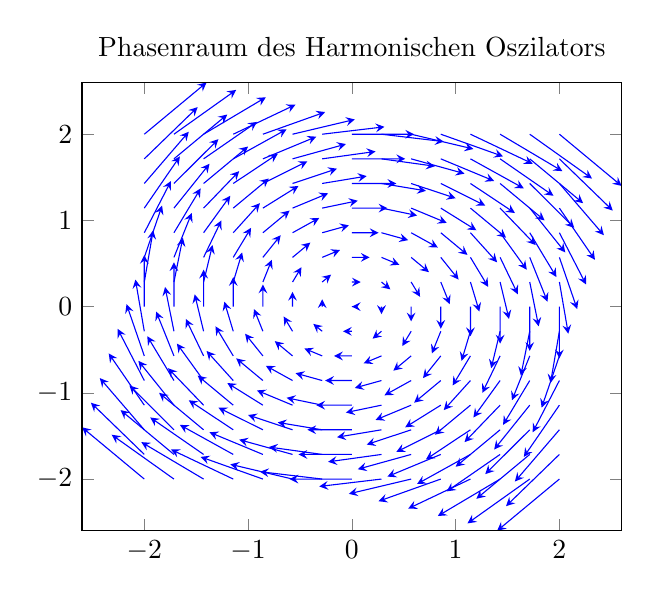
\begin{tikzpicture}
\begin{axis}[title={Phasenraum des Harmonischen Oszilators},domain=-2:2,view={0}{90},axis background/.style={fill=white}]
\addplot3[blue,quiver={u={y},v={-x},scale arrows=0.3},-stealth,samples=15] {y-x};
\end{axis}
\end{tikzpicture}
\subparagraph{Freier Fall mit Luftwiederstand}
\label{sec-3-3-9-1-4}
Aufgabe: Bestime zeitliche Entwicklung von $v$ wenn Körper im Schwerefeld losgelassen wird. $F_R = -cv^2$ \\
      Problem $1-dim$: x wachse nach unten, Start bei $t = 0, x = 0, \dot{x} = 0$
\[F=m\ddot x \Rightarrow m g - c \dot{x}^2 = m\ddot x \Rightarrow \begin{cases} m g - cv^2 &= m \dot{v} \\ v &= \dot{x} \end{cases}\]
Erste Gleichung enthält kein $x$ und kann unabhängig gelöst werden:
\begin{align*}
\frac{\d v}{\d t} &= g - \frac{c}{m}v^2 \\
\d t &= \frac{\d v}{g - \frac{c}{m}v^2}
\end{align*}
Konstanten und Dimensionen
\[[g] = \si{\meter\per\second\squared};[\frac{c}{m}] = \si{\newton\per\kilo\gram\per\meter\squared\second\squared}\]
Kann leicht Konstanten der Dimension Zeit und Geschwindigkeit bilden:
\[\hat{t} = \sqrt{\frac{m}{g c}},\hat{v} = \sqrt{\frac{g m}{c}}\]
Benutze jetzt die dimensionslosen Variablen $t' = \frac{t}{\hat{t}},v'=\frac{v}{\hat{v}}$
\[\Rightarrow \d t' = \frac{d v'}{1 - v^{2\prime}} = \frac{\d v'}{2}(\frac{1}{1 + v'} + \frac{1}{1 - v'})\]
\[2t' = \ln{1 + v'} - \ln{1 - v'} + c\]
$v' = 0$ bei $t' = 0 \Rightarrow c = 0$
Auflösen nach $v'$: \[e^{2t'} = \frac{1 + v'}{1 - v'} \Rightarrow \ldots\]
\[\Rightarrow v' = 1 - \frac{2}{e^{2t'} + 1} \Rightarrow v = \hat{v}(1 - \frac{2}{e^{\frac{2t}{\hat{t}}}} + 1)\]
$\Rightarrow$ $\hat{v}$ ist Grenzgeschwindigkeit, wird exponentiell angenommen, wenn $t \gg \hat{t}$ \\

Zugabe: einfache physikalische Argumente für die Größe von $c$:
\begin{enumerate}
\item $[c] = \si{\kilo\gram\per\meter}$, Input: $A$ (Querschnitt), $\rho_L$
         $\Rightarrow c \sim \rho_L A$
\item Energiebilanz an verdrängter Luft: \[F_R\cdot l \sim E_{\text{kin,Luft}}\sim\rho_L l A \frac{v^2}{2}\]
\end{enumerate}
\subsection{Taylorentwickung}
\label{sec-3-4}
Ohne Beschränkung der Allgemeinheit $x_0 = 0$. Untersuche Verhalten beliebiger glatter Funktionen $f(x)$ nahe $x = 0$
\begin{align*}
f(x) &= f(0) + \int_0^x\d x' f'(x') \\
&= f(0) + f'(x')(x_ - x)\Big|_0^x - \int_0^x\d x' f''(x')(x'-x) \\
&= f(0) + f'(0)x - f''(x')\frac{(x' - x)}{2}\Big|_0^x + \int_0^x\d x' f'''(x')\frac{(x' - x)^2}{2} \\
&= f(0) + f'(x)x + f''(0)\frac{x^2}{2} + \ldots
\end{align*}
Allgemein:
\[f(x) = f(0) + \sum_{n=1}^m f^{(n)}(0)\frac{x^n}{n!}+\overbrace{\int_0^x \d x' f^{(m+1)}(x')\frac{(x' - x)^m}{m!}}^{\text{Restglied}}\]
Falls das Restgliend für $n\to\infty$ verschwindet:
\[f(x) = f(0) + \sum_{n=1}^\infty f^{(n)}(0)\frac{x^n}{n!}\]
Analog:
Taylor-Reihe: \[f(x) = f(x_0) + \sum_{n=1}^\infty f^{(n)}(x_0)\frac{(x - x_0)^n}{n!}\]
\begin{enumerate}
\item Oft erste Terme = gute Näherung
\item Verallgemeinerung auf viele Variablen
\end{enumerate}
\subsubsection{Interessantes "Gegenbeispiel"}
\label{sec-3-4-1}
\[f(x) \equiv \begin{cases} e^{-\frac{1}{x^2}} & x\neq 0 \\ 0 & x = 0 \end{cases}\]
Überzeugen sie sich, dass alle Ableitungen existieren, auch bei Null! \\
    Sie Brauchen:
\[\lim_{x\to 0}\frac{1}{x^n}e^{-\frac{1}{x^2}} = 0\]
Die Ableitungen verschwinden sogar bei Null $\Rightarrow$ Taylor-Reihe ist Null, keine gute Näherung
\subsection{Harmonicher Oszillator}
\label{sec-3-5}
\begin{itemize}
\item eines der wichtigesten physikalischen Systeme
\item beschreibt viele kompilziertere Systeme angenähert
\end{itemize}
\subsubsection{Eindimensionales System}
\label{sec-3-5-1}
$d = 1, F = F(x)$
\[F(x) = -\dd{}{x}v(x) = -v'(x)\]

Damit haben wir das \textbf{Potetial} ($\rightarrow$ beschreibt die potentielle Energie des Massenpunktes) $v$ als Stammfunktion von $-F$ definiert
\begin{itemize}
\item Skizze
\end{itemize}
Massenpunkt kann nur ruhen, wo $F=0$ beziehungsweise $V'=0$. Genauer: Nur Minima (Maxima instabil). \\
\paragraph{Ziel}
\label{sec-3-5-1-1}
Untersuchung der Bewegung in der Nähe von Minimal (also bei $x\approx x_0$ wobei $v'(x_0) = 0$ gelte) \\
     $V(x)$ bei $x_0$, $V'(x_0) = 0, \abs{x - x_0}$ klein \\
     \[\Rightarrow V(x) \simeq V(x_0) + \frac{1}{2}v''(x_0)(x-x_0)^2\]
\[\Rightarrow F(x) \simeq - V''(x_0)(x-x_0)\]
\[x-x_0\equiv y \Rightarrow \underbrace{F(y) = -k y}_{\text{harmonischer Oszillator}}, k\equiv v''(0)\]
Wir sehen: Harmonischer Oszillator ist eine Idealisierung von potentiell sehr großem Nutzen (viele Systeme)
\paragraph{Lösung}
\label{sec-3-5-1-2}
Newton $\Rightarrow$ $m\ddot{y} = -ky$ beziehungsweise $\ddot{y} = -\omega^2 y,\omega\equiv\sqrt{\frac{k}{m}}$ \\
     $\Rightarrow$ $\sin{\omega t}$ und $\cos{\omega t}$ sind Lösungen \\
     $\Rightarrow$ $y(t) = A\sin{\omega t} + B\cos{\omega t}$ iist auch Lösung (wegen Linearität) \\
     (wegen der beiden frei wählbaren Konstanten ist dies schon die allgemeine Lösung)
\paragraph{Verallgemeinerungen}
\label{sec-3-5-1-3}
\begin{itemize}
\item Reibungterm $\sim \dot{y}$
\item treibende Kraft $\sim f(t)$
\end{itemize}
\subsection{Lineare Differentialgleichungen}
\label{sec-3-6}
allgemeine Form einer linearen Dgl. n-ter Ordnung:
\[y^{(n)} + f_{n -1}(x)y^{(n - 1)}(x) + \ldots + f_0(x)y(x) = f(x)\]
Das Wort linear bezieht sich nur auf $y$, nicht $x$ \\
   Die Dgl. heißt homogen falls $f(x)\equiv 0$
Homogen von Grad $p$: Ersetzung $y\to\alpha y$ führt zu Vorfaktor $\alpha p$, hier $p = 1$
\begin{itemize}
\item wir hatten oben dem Fall $n = 2$ "mit konstanten Koeffizienten"
\item noch einfacheres Beispiel: $n = 1, f\equiv 0$ (aber beliebige Koeffizienten)
\[y' + a(x)y = 0\]
Das ist seperabel:
\[\dd{y}{x} + a(x) y = 0\]
\[\dd{y}{x} = -a(x) y\]
\[\frac{\d y}{x} = -a(x) \d x\]
\[\int\frac{\d y}{y} = - \int a(x)\d x\]
\[\ln{y} - A(x) + c_1\]
\[y = c e^{-A(x)}\]
$A(x)$ sei eine beliebege aber fest gewählte Stammfunktion von $a$
Wir können den inhomogenen Fall lösen, durch "Variation der Konstanten"
\begin{itemize}
\item Ansatz: $y = C(x)e^{-A(x)}$, Dgl. $y' + ay = f$
       \[(c e^{-A})' + a C e^{-A} = f\]
       \[c' e^{-A} - C A' e^{-A} + C a e^{-A} = f\]
       Beachte $A' = a$
       \[\Rightarrow c'e^{-A} = f e^{A},c(x) = \int\d x f(x) e^{A(x)}\]
       \[y(x) = \left[\int^x\d x' f(x') e^{A(x')}\right] e^{-A(x)}\]
       $f(x')$ ist eine frei wählbare additive Konsante im $x'$-Int. ($C(x)\to C(x) +\alpha$) entspricht der Addition der Lösung der homogenen Dgl.
\end{itemize}
\end{itemize}
\subsubsection{Zusammenfassung / Verallgemeinerung auf $n > 1$}
\label{sec-3-6-1}
\begin{defn}[Linear Unabhängig]
Ein Satz von Funktionen $f_1(x),\ldots,f_n(x)$ heißt linear unabhängig, falls jede Linearkombination bei der nicht alle Koeffizienten Null sind auch nicht Null ist:
\[\alpha_1 f_1(x) +\ldots \alpha_n f_n(x)\equiv 0 \Rightarrow \alpha_1 = \ldots = \alpha_n = 0\]
(identisch zur linearen Unabhängigkeit von Vektoren)
\end{defn}
\paragraph{Fakt}
\label{sec-3-6-1-1}
Kennt man $n$ linear unabhängige Lösungen einer homogenen linearen Dgl. $n$-ter Ordnung, so kenn man die allgemeine Lösung:
\[y_{hom}(x) = C_1 y_1(x) + \ldots + C_n y_n(x)\]
Die allgeimeine Lösung ist stets von dieser Form.

Wenn wir außerdem eine \textbf{partikuläre} Lösung der onhomogenen Gleichung haben, so haben wir auch schon deren allgemeinen Lösung
\begin{align*}
y(x) = y_{hom}(x) + y_{part}(x)
\intertext{"Beweis" durch Einsetzen in}
y^{(n)} + f_{n - 1}y^{(n - 1)} + \ldots + f_0 y = f
\end{align*}
\subsubsection{Finden der partikulären Lösung}
\label{sec-3-6-2}
Auch bei $n > 1$: Variation der Konstanten (Funktioniert gut bei konstanten Koeffizienten)
Mächtigere Methoden: Überführen von System von linearen Dgl. 1. Ordnung (braucht Matrixrechnung)
\section{Erhaltungssätze in Newtonscher Mechanik}
\label{sec-4}
\subsection{Impulserhaltung}
\label{sec-4-1}
Systeme mit mehreren Massenpunkten $a,b\in\{1,\ldots, n\}$ \\
   Trajektorien: $\v x_a(t), a=1,\ldots,n$ \\
\begin{thm}[Impulserhaltung]
Bei verschwindenen externen Kräften ($\v F_{ext} = 0$) gilt:
\[\v p \equiv \sum_a \v{P_a} \equiv \sum_a m_a\dot{\v{x_a}} =~\text{const}\]
\end{thm}
\begin{proof}
\begin{align*}
\dot{\v p} &= \sum_a m_a \ddot{\v{x_a}} \\
&= \sum_a \v{F_a} \\
&= \sum_a(\sum_{\substack{b \\ a\neq b}} \v{F_{ab}}) \\
&= \sum_{\substack{a,b \\ a\neq b}} \v{F_{ab}} \tag{Summe über alle Paare von $a,b$} \\
&= \sum_{a > b}\v{F_{ab}} + \sum{a < b} \v{F_{ab}} \\
&= \sum_{a > b}(\v{F_{ab}} + \v{F_{ba}})
&\underarrow[=]{3. Newtonsches Axiom} 0 \tag*{\qedhere}
\end{align*}
\end{proof}

mit äußeren Kräften:
\[\dot{\v p} = \sum_a \v F_{a,ext.} \equiv \v F_{ext}\]
Falls zum Beispiel die äußere Kraft nicht in $x^1$ -Richtung wirkt (F$^{\text{1}}_{\text{ext}}$ = 0), so gilt immer nocht $p^1 = \text{const}$
(eigentlich drei Erhaltungssätze für \$p$^{\text{1}}$, p$^{\text{2}}$,p$^{\text{3}}$, manchmal gelten nur einige davon)
\subsection{Drehimpusherhaltung}
\label{sec-4-2}
Oft: Kräfte wirken parallel zur Verbindungslinie zweier Massenpunkte:
\begin{itemize}
\item Gravitationskraft
\item Elektrostatitsche Kraft
\item Modell der masselosen Stange ($\rightarrow$ Modell für starre Körper!)
\end{itemize}
\begin{defn}[Drehimpuls]
\begin{align*}
\v L_a &\equiv \v x_a \times \v p_a \\
(\v L_a)^i &= \varepsilon^{ijk}x_a^j p_a^k
\end{align*}
\end{defn}
Falls $\v F_{a,ext} = 0$ und alle interen Kräfte wirken parallel zur Verbindungslinie der jeweiligen Punkte, dann gilt \textbf{Drehimplusherhaltung}
\begin{thm}[Drehimpulserhaltung]
\[\v L \equiv \sum_a \v L_a = \sum_a m_a \v x_a \times \dot{\v x}_a = \sum_a \v x_a \times \v p_a = ~\text{const}\]
\end{thm}
\begin{proof}
Nachrechnen:
\begin{align*}
\dot{\v L} &= \sum_a m_a (\dot{\v x}_a \times \dot{\v x}_a + \v x_a + \ddot{\v x}_a) \\
&= \sum_a \v x_a \times \v F_a \\
&= \sum_{a\neq b} \v x_a \times \v F_{ab} \tag{Summe über alle Paare von $a,b, a\neq b$} \\
&= \sum_{a > b}(\v x_a \times \v F_{ab} + \v x_b \times \v F_{ba}) \\
&= \sum_{a > b} (\v x_a - \v x_b)\times \v F_{ab} \\
\intertext{da $\v F_{ab} \parallel (\v x_a - \v x_b)$ per Annahme} \\
&= 0 \tag*{\qedhere}
\end{align*}
\end{proof}
Bei externen Kräften:
\[\dot{\v L} = \sum_a \v x_a \times \v F_{a,ext} \equiv \v M_{ext}\]
$M_{ext}$ ist das durch äußere Kräfte auf Punkt $a$ ausgeübte \textbf{Drehmoment}, allgemein (für einzelnen Punkt):
\[\v M = \v x \times \v F = \dot{\v L}\]

Wichtig: Drehimpulserhaltung gilt auch dann wenn alle äußeren Kräfte \textbf{Zentralkräfte} sind, Zentralkraft:
\[\v F_a \parallel \v x_a\]

Drehimpuls hängt vom Koordinatensystem ab.
\begin{remark}
$\v L \equiv \v x\times \v p$ (allgemeiner jedes Kreuzprodukt von Vektoren) \\
ist ein \textbf{Axial-} oder \textbf{Pseudovektor}, das heißt: Bei Drehungen wei Vektor, Bei Reflexion an ursprung kein Vorzeichenänderung
\begin{proof}
\[\v a \to -\v a, \v b \to -\v b \Rightarrow \v a \times \v b \to + \v a \times \v b \qedhere\]
\end{proof}
\end{remark}
\subsection{Konservative Kräfte und Energieerhaltung}
\label{sec-4-3}
\begin{defn}[Gradient]
Gradient von $V$:
\[\v\nabla \equiv \left(\frac{\partial V}{\partial x^1}, \frac{\partial V}{\partial x^2}, \frac{\partial V}{\partial x^3}\right)\]
$\frac{\partial}{\partial x}$ ist ein "Differentialoperator", also:
\[\frac{\partial}{\partial x}:f(x,y)\mapsto \frac{\partial f(x,y)}{\partial x}\]
Dementsprechen $\frac{\partial^2}{\partial x^2}$ ist ein "Differentialoperator" zweiter Ordung, also:
\[\frac{\partial^2}{\partial x^2}:f(x,y)\mapsto \frac{\partial^2 f(x,y)}{\partial x^2}\]
$\v\nabla V$ ist gute Schreibweise, weil $\v\nabla$ ein vektorwertiger Differentialoperator ist:
\[\v\nabla = \left(\frac{\partial}{\partial x^1}, \frac{\partial}{\partial x^2}, \frac{\partial}{\partial x^3}\right)\]
\end{defn}
\begin{defn}[konservatives Kraftfeld]
Ein zeitunabhängiges Kraftfeld $\v F(\v x)$ heißt \textbf{konservativ} falls es eine Funktion $V(\v x)$ ("Potential") gibt. dodass
\[\v F = -\v \nabla V\]
\end{defn}
\subsubsection{Energieerhaltung}
\label{sec-4-3-1}
Für einen Massenpunkt in einem konservativen Kraftfeld gilt:
\[E = \underset{\text{kinetisch}}{T} + \underset{\text{potentielle Energie}}{V} = \frac{m}{2}\dot{\v x}(t)^2 + V(\v x(t)) = \text{const}\]
\paragraph{Begründung}
\label{sec-4-3-1-1}
\begin{align*}
\dd{T}{t} &= \frac{m}{2}\dd{}{t}(\dot{x}^i\dot{x}^i) = \frac{m}{2}2 \dot{x}^i \ddot{x}^i = m\dot{\v x}\ddot{\v x} \\
\dd{V}{t} &= \lim_{\Delta t \to 0} \frac{V(x^1 + \Delta x^1, x^2 + \Delta x^2, x^3 + \Delta x^3) - V(x^1, x^2, x^3)}{\Delta t} \\
\intertext{mit $\Delta x = \dd{\v x}{t}\Delta t$} \\
\intertext{Umschreiben des Zählers} \\
&V(x^1 + \Delta x^1, x^2 + \Delta x^2, x^3 + \Delta x^3) - V(x^1, x^2 + \Delta x^2, x^3 + \Delta x^3) \\
+ &V(x^1, x^2 + \Delta x^2, x^3 + \Delta x^3) - V(x^1, x^2, x^3 + \Delta x^3) \\
+ &V(x^1, x^2, x^3 + \Delta x^3) - V(x^1, x^2, x^3) \\
&\cong \frac{\partial V}{\partial x^1}(x^1,x^2 + \Delta x^2, x^3 + \Delta x^3)\Delta x^1 + \frac{\partial V}{\partial x^1}(x^1,x^2,x^3 + \Delta x^3) \Delta x^2 + \frac{\partial V}{\partial x^1} (\v x)\Delta x^3
\intertext{Teilen durch $\Delta t$, Grenzwertbildung}
\dd{V}{t} &= \frac{\partial V}{\partial x^i}(\v x(t))\dd{x^i}{t} \\
\shortintertext{oder (allgemeine Rechenregel)}
\d V &= \frac{\partial V}{\partial x^i} \d x^i
\end{align*}
Allgemeine Formulierung der Rechenregel: Sei $f:\mathbb{R}^n \to\mathbb{R} \wedge \v x: \mathbb{R}\to\mathbb{R}^n$
Die Verknüpfung $f\circ \v x: \mathbb{R}\to \mathbb{R}$ ist eine Funktion. Für diese gilt:
\begin{align}
\underbrace{\d f}_{\mathclap{\text{totales Differential}}} &= \frac{\partial f}{\partial x^i}\d x^i = (\v\nabla f) \d \v x \\
\shortintertext{oder totale Ableitung:} \\
\dd{f}{t} &= \frac{\partial f}{\partial x^i} \frac{\d x^i}{\d t} \\
\shortintertext{Unsere Anwendung} \\
\dot{E} = m\dot{\v x} \ddot{\v x} + \frac{\partial V}{\partial x^i} \dot{x}^i = \v F \dot{\v x} + (\v\nabla V)\dot{\v x} = 0~\checkmark
\end{align}
\[V(x^1 + \Delta x^1, x^2 + \Delta x^2, x^3 + \Delta x^3) - V(x^1, x^2 + \Delta x^2, x^3 + \Delta x^3)\]
Vergleiche:
\[f(x + \Delta) - f(x) \cong f'(x)\Delta\]
\subsubsection{Kriterium für Konservativität}
\label{sec-4-3-2}
Für *einfach zusammenhängende Gebiete*\footnote{Jede geschlossene Kurve kann auf Länge Null zusammengezogen werden} gilt:
\[\v F ~\text{ist konservativ}~ \Leftrightarrow \v\nabla\v F = 0\]
\paragraph{Begründung}
\label{sec-4-3-2-1}
$\Rightarrow$ \\ \[\v F = -\v\nabla V \Rightarrow \underbrace{\v\nabla\times\v F}_{\mathclap{\equiv~\text{Rotation von $F$ ($\rot{F}$)}}} = 0\]
\begin{align*}
(\v\nabla\times\v F)^i &= \varepsilon^{ijk} \frac{\partial}{\partial x^j} F^k = \varepsilon^{ijk}\partial^i F^k \\
&= -\varepsilon^{ijk}\partial^j\partial^k V = -\frac{1}{2}(\varepsilon^{ijk} -\varepsilon^{ikj})\partial^j\partial^k V \\
&= - \frac{1}{2}\varepsilon^{ijk}\partial^j \partial^k V + \frac{1}{2}\varepsilon^{ikj}\underbrace{\partial^k\partial^j}_{\mathclap{\text{habe benutzt}~\frac{\partial}{\partial x}\frac{\partial}{\partial y} = \frac{\partial}{\partial y}\frac{\partial}{\partial x}}} V \\
&\underarrow[=]{$k \leftrightarrow j$} -\frac{1}{2}\varepsilon^{ijk}\partial^j\partial^k V + \frac{1}{2}\varepsilon^{ijk}\partial^j\partial^k V = 0
\end{align*}
$\Leftarrow$ \\
     Wähle beliebiges festes $\v x_0$ im Gebiet. Definiere Potential als minus Arbeit am Massenpunkt $\rightarrow Abbildung$
\begin{align*}
V(\v x) &\equiv -\int_{\v x_0}^{\v x} \v F(x)\d\v s \tag{Linienintegral} \\
\intertext{Linienintegral kann immer definiert werden, wenn Kurve durch Gebiet mit Vektorfeld verläuft}
\d\v s &\equiv \d\v x(s) =(\dd{x^1}{\d x}, \dd{x^2}{\d x}, \dd{x^3}{\d x}) \d s \\
\intertext{Also gilt:}
\v F\d\v s &= \underbrace{F^i (\dd{x^i}{s})\d s}_{\mathclap{\text{Integrand im normalen Riemann Inegral}}} \\
\intertext{Wähle beliebigen kleinen Vektor $\v l$ und berechne:}
\v l \v F(\v x) &\cong -(-\int_{\v x}^{\v x + \v l} \d\v s \v F) \\
&= -((-\int_{\v x_0}^{\v x + \v l} \d \v s \v F) - ( -\int_{\v x_0}^{\v x} \d\v s \v F)) \\
&= -(V(\v x + \v l) -V(\v x)) \\
&\cong - \frac{\partial V}{\partial x^i}l^i = -\v l(\v\nabla V) \\
&\Rightarrow \v l(\v F + \v\nabla V) = 0 \\
&\Rightarrow \v F + \v\nabla V = 0 \checkmark
\end{align*}
Lücke: Wegunabhängigketi der Definition von $V$: \\
     Wähle zwei unterschiedliche Wege ($L_1, L_2$):
\begin{align*}
\int_{L_1}\d\v s \v F - \int_{L_2}\d \v s \v F = \underarrow[\oint]{\text{Rand von } $\Sigma$} \d\v s\v F \\
\intertext{Satz von Stokes}
&= \int_{\Sigma}\v{d f}(\v\nabla \times\v F)
\end{align*}
\[(\rot \v F)^i = (\v\nabla \times \v F)^i = \varepsilon^{ijk}\frac{\partial}{\partial x^j} F^k\]
zum Beispiel:
\[(\v\nabla\times\v F)^1 = \frac{\partial F^3}{\partial x^2} - \frac{\partial F^2}{\partial x^3}\]
\[\int_{L_2}\d \v s \v F - \int_{L_1}\d \v s\v F = \oint_{\partial \Sigma} \d\v s \v F \underarrow[=]{\text{"Stokes"}} \int_{\Sigma}\d\v f*(\v\nabla\times\v F) \overset{!}{=} 0\]
\subsection{Satz von Stokes}
\label{sec-4-4}
\begin{defn}[Satz von Stokes]
\[\oint \d \v s\v F = \int_{\Sigma} \d \v f (\v \nabla \times \v F)\]
\end{defn}
\begin{proof}
\begin{align*}
\oint \d\v s\v F &= \int_0^{\Delta x^1}\d s F^1(x,0) + \int_0^{\Delta x^2}\d s F^2(\Delta x^1, s) - \int_0^{\Delta x^1}\d s F^1(s, \Delta x^2) - \int_0^{\Delta x^2}\d s F^2(0,s) \\
&= \int_0^{\Delta x^1}\d s(F^1(s,0) - F^1(s,\Delta x^2)) + \int_0^{\Delta x^2}\d s(F^2(\Delta x^1, s) - F^2(0,s)) \\
&= \int_0^{\Delta x^1}\d s(\frac{\partial F^1}{\partial x^2})\Delta x^2 + \int_0^{\Delta x^2}\d s \frac{\partial F^2}{\partial x^1}\Delta x^1 + O(\Delta^3) \\
&= \Delta x^1 \Delta x^2(\frac{\partial F^2}{\partial x^1} - \frac{\partial F^1}{\partial x^2}) + O(\Delta^3) \\
&= \Delta x^1 \Delta x^2(\v\nabla \times \v F)^3 + O(\Delta^3) \\
&= \underbrace{\Delta x^1 \Delta x^2 \hat{e_3}}_{\mathclap{\Delta \v f = ~\text{Der dem kleinen Flächenelement zugeordnete Vektor}}} (\v\nabla \times \v F) \\
&\approx \Delta \v f(\v \nabla \times \v F)
\end{align*}
Allgemein steht $\Delta \v f$ oder $\d \v f$ für ein kleines oder infinitesimales Flächenelement, Länge $\estimates$ Größe der Fläche
Die Richtung des Vektors definiert \textbf{Orientierung} der Fläche (Zum Beispiel Oben = da, wo der Pfeil hinzeigt) \\
   Randkurve: so definiert, dass man von oben gesehen linksherum (mathematisch positiver Drehsinn) läuft
\begin{enumerate}
\item Spezielle Lange in unsererer Rechung unwichtig
\item Übergang zu größeren Flächen durch Aufaddieren
\end{enumerate}
Fläche $= N\Delta ^2 \Rightarrow N\sim \frac{1}{Delta^2}$
\begin{align*}
\sum_{\text{Rechtecke}} \oint\d \v s\v F = \sum_{\text{Rechtecke}} \int\d\v f(\v\nabla \times \v F) + \underarrow[N]{Zahl der Rechtecke = $O(\Delta)$} O(\Delta^3) \\
\shortintertext{weil sich nicht "innere Ränder wegheben"}
\oint\d \v s\v F = \sum_{\text{Rechtecke}} \int\d\v f(\v\nabla \times \v F) \\
\shortintertext{klar}
\oint\d \v s\v F = \int\d\v f(\v\nabla \times \v F) \\
\end{align*}
Glätten des Randes:
Zerlegung des Randes $\Delta \v s$ in kleine Rechtecke $\Delta \v s_1, \Delta \v s_2$
\begin{align*}
\Delta \v s &= \Delta \v s_1 + \Delta \v s_2 \\
\v F \Delta\v s &= \v F \Delta \v s_1 + \v F \Delta \v s_2 = \v F_1 \Delta \v s_1 + \v F_2 \Delta \v s_2 + O(\Delta x^2)
\end{align*}
$\v F, \v F_1, \v F_2$ jeweils am Mittelpunkt der Linienelemente
Zahl derartiger Randelemente $\sim \frac{1}{\Delta} \Rightarrow$ Fehler $O(\Delta)$ \\
   $\Rightarrow$ Auch nach Summation bleibt Fehler von $O(\Delta)$

Besser wäre Zerlegung in Simplices ("Haben sie mal versucht eine Schildkröte zu fliesen")
\end{proof}

Für unsere Anwendung: wichtig, dass jede geschlossene Kurve inn einem einfach zusammenhängenden Gebiet, \textbf{Rand} ist.
\subsection{Energieerhaltung für Systeme von Massenpunkten}
\label{sec-4-5}
Massenpunkte: $\v x_a, a = 1,\ldots, n$ \\
   Kräfte: seien $\parallel$ zu $\v x_a - \v x_b$ ("Zentralkräfte") \\
   Solche Kräfte kann man stets schreiben als:
\begin{align*}
\v F_{ab} = -\v\nabla_a V_{ab}(\abs{\v x_a - \v x_b}) \\
\shortintertext{mit:}
V_{ab} = V{ba}, \v\nabla_a = (\frac{\partial}{\partial x^1_a}, \frac{\partial}{\partial x^2_a}, \frac{\partial}{\partial x^3_a}) \\
\shortintertext{dazu:}
-\v\nabla_a V_{ab} (\abs{\v x_a - \v x_b}) &= (-\v\nabla_a \abs{\v x_a - \v x_b}) V_{ab}'(\abs{\v x_a - \v x_b}) \\
\shortintertext{Dies zeigt:}
&= -\v\nabla_a \sqrt{(\v x_a - \v x_b)^2} \\
&= \frac{\v x_a - \v x_b}{\abs{\v x_a - \v x_b}}
\end{align*}
Wir können passendes $V$ für jede Zentralkraft finden. Man berechnet einfach $V'$ und sucht die Stammfunktion.

Prüfe Konsistenz mit 3. Axiom:
\[\underbrace{-\v\nabla_a V_{ab}(\abs{\v x_a - \v x_b})}_{\v F_{ab}} = + \v\nabla_b V_{ab}(\abs{\v x_a - \v x_b}) = \underbrace{+ \v\nabla_b V_{ba}(\abs{\v x_b - \v x_a})}_{-\v F_{ba}}\]

In diesem System gilt Energieerhaltung:
\[E = \sum_a T_a + \frac{1}{2}\sum_{a\neq b} V_{ab} = \sum_a T_a + \sum_{a < b} V_{ab} = ~\text{const}\]

Begründung:
\begin{align*}
\dot{E} &= \sum_a \dot{\v x}_a \v F_a + \frac{1}{2}\sum_{a\neq b}((\v \nabla_a V_{ab})\dot{\v x}_a + (\v\nabla_b V_{ab})\dot{\v x}_b) \\
&= \sum_{a\neq b} \dot{\v x}_a \v F_{ab} + \frac{1}{2}\sum_{a\neq b} ( -\v F_{ab}\dot{\v x}_a - \underbrace{\v F_{ab} \dot{\v x}_b}_{\mathclap{\text{Umbennenung $a\leftrightarrow b$}}}) = 0 \\
(& = W - \frac{1}{2} W - \frac{1}{2} W)
\end{align*}

Bemerkung: Passend gewähltes $V_{ab}$ gibt das Modell der starren Stangen
\subsection{Eindimensionale Bewegung}
\label{sec-4-6}
\[F(x) = m\ddot{x}\]
\begin{itemize}
\item mit Einsatz allgemein lösbar!
\item Startpunkt: Jedes 1-dim. zeitunabhängiges Kraftfelt ist konservativ
\begin{align*}
E = \frac{m}{2}\dot{x}^2 + V(x) = ~\text{const} \\
\intertext{(bis auf Vorzeichen)}
\dot{x} = \sqrt{\frac{2}{m}(E-V(x))} \Rightarrow \d t = \frac{\d x}{\sqrt{\frac{2}{m}(E-V(x))}} \\
t = \in \frac{\d x}{\sqrt{\frac{2}{m}}(E - V(x))}
\intertext{Integral lösen, Integrationskonstante und Energie so bestimmen, das Anfangswertproblem gelöst}
t = t(x) ~\text{auflösen}~ \Rightarrow x = x(t) \checkmark
\intertext{viel einfacher als allgemeine Differentialgleichung 2. Ordnung}
\end{align*}
\end{itemize}
\section{Harmonischer Oszillator in komplexen Zahlen}
\label{sec-5}
\subsection*{Motivation}
   Harmonischer Oszillator mit Reibung:
   \[\ddot{x} = -\omega^2 x - c \dot{x}\]
   Exponentieller Ansatz:
   \[x\sim e^{\alpha t} \Rightarrow \alpha^2 + \omega^2 + c\alpha = 0\]
   gesucht: $\alpha$, Betrachte Genzfälle:
\begin{enumerate}
\item $\omega$ klein
\[\Rightarrow \alpha^2 + c\alpha = 0 \Rightarrow \alpha = -c \Rightarrow x\sim e^{-c t}\]
\item $\omega$ groß (beziehungsweise $c$ klein)
\[\alpha^2 + \omega^2 \simeq 0\]
nicht lösbar!
\end{enumerate}
Aber: wir wissen schon $\sin{\omega t}, \cos{\omega t}$ sind Lösungen.

Falls jede gesuchte Gleichung lösbar $\Rightarrow$ Hoffnung auf elegante allgemeine Lösung

\textbf{Speziell:} $\alpha^1 = -1$ (für $\omega = 1, c = 0$)
\subsection{Komplexe Zahlen}
\label{sec-5-1}
\subsubsection{Ziel}
\label{sec-5-1-1}
reelle Zahlen so zu erweitern, dass $x^2 = - 1$ lösbar
\subsubsection{Naive Definition}
\label{sec-5-1-2}
Definiere "Imaginäre Einheit" $x^2 = -1$ lösbar "$\I$", so dass $\I^2 = -1$
Wollen addieren und Multiplizieren, deshalb erkläre komplexe Zahl $\mathbb{C}$ als:
\[\mathbb{C} \ni z ) x + \I y, x,y\in\mathbb{R}\]
Wir definieren außerdem:
\begin{itemize}
\item $z_1 + z_2 = (x_1 + \I y_1) + (x_2 + \I y_2) \equiv (x_1 + x_2) + \I(y_1 + y_2)$
\item $z_1 \cdot z_2 = (x_1 + \I y_1) (x_2 + \I y_2) \equiv x_1 x_2 + x_1 \I y_2 + \I y_1 x_2 + \I y_1 \I y_2 \equiv (x_1 x_2 - y_1 y_2) + i(x_1 y_2 + x_2 y_1)$
\end{itemize}
\subsubsection{präsizere Definition}
\label{sec-5-1-3}
\begin{defn}[Körper]
Körper ("Field") ist eine Menge $K$ mit zwei binären Operationen $("+","\cdot")$, so dass:
\begin{itemize}
\item $\alpha + (\beta + \gamma) = (\alpha + \beta) + \gamma$ \hfill (Assoziativität)
\item $\alpha + \beta = \beta + \alpha$ \hfill (Kommutativität)
\item $\Exists 0 \in K: \alpha + 0 = \alpha \Forall \alpha$ \hfill (Null)
\item $\Forall \alpha \Exists (-\alpha) \in K: \alpha + (-\alpha) = 0$ \hfill (Additives Inverses)
\item $(\alpha \cdot \beta) \cdot \gamma = \alpha \cdot (\beta \cdot \gamma)$ \hfill (Assoziativität der Mult.)
\item $\alpha \cdot \beta = \beta \cdot \alpha$ \hfill (Kummutativität der Mult.)
\item $\Exists 1 \in K: 1\cdot \alpha = \alpha \Forall \alpha$ \hfill (Eins)
\item $\Forall \alpha \neq 0 \Exists \alpha^{-1} \in K: \alpha \cdot \alpha^{-1} = 1$ \hfill (Inverses der Mult.)
\item $\alpha\cdot (\beta + \gamma) = \alpha \cdot \beta + \alpha \cdot \gamma$ \hfill (Distributivität)
\end{itemize}
\end{defn}
Wir kennen bereits:
\begin{itemize}
\item $K = \mathbb{Q}$ \hfill (rationale Zahlen)
\item $K = \mathbb{R}$ \hfill (reelle Zahlen)
\end{itemize}
\begin{defn}[Komplexer Zahlenkörper]
Komplexe Zahlen sind die Menge $\mathbb{C} = \mathbb{R} \times \mathbb{R} = \mathbb{R}^2$ mit den Operationen
\begin{itemize}
\item $(x_1, y_1) + (x_2, y_2) \equiv (x_1 + x_2, y_1 + y_2)$
\item $(x_1, y_1) \cdot (x_2, y_2) \equiv (x_1 \cdot x_2 - y_1 \cdot y_2, x_1 \cdot y_2 + x_2 \cdot y_1)$
\end{itemize}
Das ist äquivalent zu unserer "naiven Definition" $z = x + \I y$
\end{defn}
\textbf{Aufgabe:} Prüfen sie, dass die Axiome erfült sind! \\
    Schwierigster Teil: Multiplikations-Inverses, Idee / Vorschlag:
\[z^{-1} = (x + \I y)^{-1} = \frac{x}{x^2 + y^2} - \I \frac{y}{x^2 + y^2}\]

$\mathbb{C} = \mathbb{R}^2 \Rightarrow$ Darstellung durch Vektoren in Ebene liegt nahe.
\begin{itemize}
\item Addition: $\equiv$ Vektoraddition
\item Multiplikatoin: Beträge der Vektoren werden multipliziert, Winkel "$\arg$" werden addiert.
\item $\arg{z} = \phi$
\item $\Re{z} = x$
\item $\Im{z} = y$
\item $\abs{z} = \sqrt{x^2 + y^2}$
\end{itemize}

Übliche Funktionen ($\exp, \ln, \sin, \cos$) können mittels ihrer in $\mathbb{R}$ bekannten Taylorreihe auf $\mathbb{C}$ übertragen werden \\
    \textbf{Besonders wichtig:}
\[e^z \equiv \sum_{n = 0}^\infty \frac{z^n}{n!}\]
Brauchen $e^{z + w} = e^z \cdot e^w$ \\
    Nachrechnen:
\begin{align*}
e^{z + w} &= \sum_{n = 0}^\infty \frac{(z + w)^n}{n!} = \sum_{n = 0}^\infty \frac{1}{n!}\sum_{k = 0}^n \underarrow[\binom{n}{k}]{$\mathclap{\underset{\binom{n}{k} = \frac{n!}{k!(n -k)!}}{\text{Binomialkoeffizient}}}$} z^kw^{n - k}
\intertext{englisch: "n choose k"}
\intertext{durch Umschreiben der Summen erhält man:}
&= \sum_{n = 0}^\infty \sum_{k = 0}^n \frac{n^k}{k!} \frac{w^{n -k}}{(n -k)!} \\
&= \sum_{k = 0}^\infty \sum_{l = 0}^\infty \frac{z^k}{k!} \frac{w^l}{l!} = e^z e^w
\end{align*}
Insbesondere:
\[e^z = e^{x + \I y} = \underbrace{e^x}_{\mathclap{\text{reelle Zahl}}} \overbrace{e^{\I y}}^{\mathclap{\text{komplexe Zahl e vom Betrag $1$}}}\]
In der Tat:
\begin{align*}
e^{\I y} &= \sum_{n = 0}^\infty \frac{(\I y)^n}{n!} = \sum_{k = 0}^\infty \frac{\I y^{2 k}}{(2 k)!} + \sum_{k = 0}^\infty \frac{(\I y)^{2k + 1}}{(2 k + 1)!} \\
&= \sum_{k = 0}^\infty \frac{(-1)^k y^{2k}}{(2 k)!} + \I \sum_{k = 0}^\infty \frac{(-1)^k y^{2k + 1}}{(2k + 1)!} \\
&= \cos{y} + \I \sin{y}
\end{align*}
$\Rightarrow$ Eulersche Formel
\[e^{\I \phi} = \cos{\phi} + \I \sin{\phi}\]
\subsubsection{Zusammenfassung:}
\label{sec-5-1-4}
\[e^{\I\phi} = \cos{\phi} + \I \sin{\phi}\]
\[w = e^z = e^x e^{\I y} = \abs{w}e^{i\arg{w}}\]
\[\ln{w} = z = x + \I y = \ln{\abs{w}} + \I \arg{w}\]
Problem: $\arg{w}$ und deshalb $\ln$ nicht eindeutig definiert \\
   Lösung: Definiere $\arg{w} \in (-\pi, \pi)$

\subsubsection{Fundamentalsatz der Algebra}
\label{sec-5-1-5}
In $\mathbb{C}$ hat jedes Polynom
\[P_n(z) = \sum_{i = 0}^n a_i z^i\]
eine Nullstelle $z_0$

In der Tat hat es sogar $n$ Nullstellen:
\[P_n(z) = (z - z_0)\cdot \underbrace{P_{n - 1}(z)}_{\mathclap{\text{Hat wieder eine Nullstelle, usw.}}}\]

(Man sagt: Körper $\mathbb{C}$ ist algebraisch abgeschlossen)
\begin{itemize}
\item Es gibt auf $\mathbb{C}$ wichtige Abbildung: "komplexe Konjugation"
\[z \to z^\ast \estimates z\to \bar z\]
Definiert durch:
\[(x + \I y)^\ast = x - \I y, (\rho e^{\I \phi})^\ast = \rho e^{-\I \phi}\]
also auch
\[(z^\ast)^\ast = z\]
\end{itemize}
\subsubsection{Quaternionen}
\label{sec-5-1-6}
\[1,i \to 1,i,j,k, i^2 = j^2 = k^2 = -1\]
\[ij = k, j i = -k, jk = i,\ldots\]
\subsection{Anwendung auf harmonischen Oszillator}
\label{sec-5-2}
\begin{align*}
\intertext{Erinnerung: pyhsikalisches Problem:}
\ddot{x} + c \dot{x} + \omega^2 x = 0 \\
\intertext{Fall $\frac{c}{2} > \omega$ (Kriechfall)}
x=e^{\alpha t}, \alpha^2 + c\alpha + \omega^2 = 0 \\
\alpha_{1,2} =-\frac{c}{2} \pm \sqrt{\frac{c^2}{4} - \omega^2} \\
\intertext{$\Rightarrow$ 2 linear unabhängige Lösungen, also allgemeine Lösung durch linare Superposition}
\intertext{$\Rightarrow$ exponentielles Abfallverhalten, ohne Oszillationen}
\intertext{Fall $\frac{c}{2} < \omega$ (Schwingfall), $\sqrt{-x} = \I \sqrt{x}$}
\alpha_{1,2} = -\frac{c}{2}\pm \I\sqrt{\omega^2 - \frac{c^2}{4}} \equiv -\frac{c}{2} \pm \I \tilde\omega \\
x_{1,2} = e^{-\frac{c}{2}t} e^{\pm \I \omega t} = e^{-\frac{c}{2}t} (\cos{\pm \tilde \omega t} + \I \sin{\pm\tilde\omega t}) \\
x_{1,2} =  e^{-\frac{c}{2}t} (\cos{\tilde \omega t} \pm \I \sin{\tilde\omega t}) \\
\intertext{Durch Linearkombination $\to$ 2 reelle Lösungen:}
x_1 = e^{-\frac{c}{2}t}\cos{\tilde \omega t};\qquad x_2 = e^{-\frac{c}{2}t} \sin{\tilde\omega t}
\intertext{$\Rightarrow$ allgemeine Lösung durch Linearkombination}
\intertext{$\Rightarrow$ gedämpfte Schwingung}
\intertext{Fall $\frac{c}{2} = \omega$ (aperiodischer Grenzfall)}
\alpha_1 = \alpha_2
\intertext{$\Rightarrow$ Nur eine linear unabhängige Lösung, brauche weitere Lösung um allgemeine Anfangsbedinungen zu erfüllen}
\intertext{Idee: Betrachte Schwingfall Lösungen für $\tilde \omega \to 0$}
\intertext{Taylor:}
\cos{x} = 1 + \O(x^2);\qquad \sin{x} = x + O(x^3) \\
\Rightarrow x_1 = e^{-\frac{c}{2}t}; \qquad x_2 = e^{-\frac{c}{2}t} \tilde\omega t
\intertext{$\Rightarrow$ Wieder asymptotische Annäherung an $0$ ohne Oszillation}
\end{align*}
\subsection{harmonischer Oszillator mit periodisch treibender Kraft}
\label{sec-5-3}
\begin{align*}
\intertext{Inhomogene Dgl:}
\ddot{x} + c \dot{x} + \omega^2 x = \frac{1}{m} F(t), F(t) = f e^{\I \ubar\omega t}  \\
\intertext{Ansatz:}
x(t) = A e^{\I \ubar \omega t} \\
\Rightarrow (A (-\ubar\omega^2 + \I c \ubar\omega + \omega^2) - \frac{f}{m}) e^{\I \omega t = 0} \\
A \equiv \abs{A}e^{\I \phi} = \frac{f}{m}\cdot\frac{1}{\omega^2 - \ubar\omega^2 + \I c \ubar \omega} \\
\intertext{mit}
\frac{1}{a + \I b} = \frac{a - \I b}{a - \I b} \frac{1}{a + \I b} = \frac{a - \I b}{a^2 - b^2} \\
\intertext{und elementarer Algebra findet man den Realteil der Lösung:}
\Re x(t) = \abs{A} \cos{\ubar \omega t + \phi} \\
\abs{A} = \frac{\frac{f}{m}}{\sqrt{\omega^2 - \ubar \omega^2} + c^2 \ubar\omega^2}, \tan{\phi} = \frac{c\ubar\omega}{\ubar\omega^2 - \omega^2}
\end{align*}
Allgemeine Lösung ergibt sich, indem man zu dieser partikulären Lösung der inhomogenen Gleichung die allgemeine Lösung der homogenen Gleichung addiert.

Wichtig: Langzeitverhalten ist durch die partikuläre Lösung bestimmt $\Rightarrow$ Resonanzkatastrophe bei $c \to 0 \& \ubar \omega \to \omega$
% Emacs 25.1.1 (Org mode 8.2.10)
\end{document}